% Szablon dokumentu został pobrany z https://ii.uni.wroc.pl/dla-studenta/prace-dyplomowe
\documentclass[shortabstract,inz]{iithesis}
\usepackage[utf8]{inputenc}

\polishtitle{Organizacja oraz prowadzenie gier fabularnych zdalnie z pomocą autorskiego bota na serwerze Discord}
\englishtitle{Organizing and management of role-playing games remotly using custom made bot on Discord server}
\polishabstract{
Celem niniejszej pracy inżynierskiej była implementacja aplikacji \textit{RPGamer} potocznie zwanej \textit{botem}, mającej znacznie uprościć organizację i prowadzenie wydarzeń (w szczególności \textit{Sesji RPG}), zrzeszających określoną grupę osób. Projekt działa na serwerze komunikatora Discord uczestników, a jego funkcje wywoływane są przy pomocy komend na czacie tekstowym. Bot jest aplikacją napisaną w sposób asynchroniczny, z użyciem biblioteki \textit{discord}, korzystającą z biblioteki \textit{SQLAlchemy}, która stosuje podejście ORM dla bazy danych \textit{SQLite}. Projekt wykorzystuje istniejące mechanizmy komunikatora Discord, w celu implementacji nowych narzędzi przystępnych dla użytkowników. Zaimplementowano m.in rzucanie kostką przez gracza, podsumowywanie wyników rzutów po wydarzeniu, tworzenie ankiet dla graczy czy obsługę odtwarzania plików dźwiękowych z serwisu YouTube.

}
\englishabstract{Abstract in english - It's going to be written after the whole paper is finished.}
\author{Mateusz Zając}
\advisor{dr Marcin Młotkowski}

%\date{}
\transcriptnum{298654}
\advisorgen{dr Marcina Młotkowskiego}

% miejsce na dodatkowe pakiety
\usepackage{graphicx}
\usepackage{caption}
\usepackage{subcaption}
% this one is mandatory to ensure biblatex working without warnings
\usepackage{csquotes}
\usepackage[backend=biber]{biblatex}
\usepackage{listings}
\usepackage[lstlisting]{totalcount}

% miejsce na własne polecenia itd
\graphicspath{{./pics}}
\addbibresource{biblio.bib}
\newcommand*\lstinputpath[1]{\lstset{inputpath=#1}}
\lstinputpath{code}
\emergencystretch=1em
\lstset{
	numbers=left,
	stepnumber=1,
	breaklines=true,
	showstringspaces=false,
	basicstyle=\footnotesize,
	tabsize=1,
	breakatwhitespace=false,
	xleftmargin=5.0ex
}
\newcommand\conditionalLoL{%
	\iftotallstlistings\lstlistoflistings\fi}
\renewcommand\lstlistlistingname{Listingi}

\begin{document}
	\chapter*{Wstęp}
		\addcontentsline{toc}{chapter}{Wstęp}
		Społeczności nie zawsze są w stanie spotkać się w świecie rzeczywistym, co stawia je przed wyborem sposobu zdalnej konwersacji oraz wymiany informacji. Podczas gdy proste spotkania można szybko i łatwo zorganizować na dowolnym komunikatorze, tak rozgrywanie \textit{Sesji RPG}\cite{sesjarpg} na odległość nie jest już do końca trywialne. Szybko okazuje się, że prosty komunikator głosowy łączący uczestników bardzo ogranicza możliwości oraz jest w stanie istotnie obniżyć immersję świata przedstawionego względem rzeczywistych rozgrywek. Brakuje programowych mechanizmów, które wspomagałyby podobne wydarzenia i wyręczały uczestników w powtarzalnych i żmudnych operacjach. Dostępne na rynku gotowe produkty często nie łączą wszystkich pożądanych funkcjonalności, a korzystanie z wielu rozwiązań jednocześnie w celu realizacji zamierzonych celów jest dla użytkowników uciążliwe. 
		
		\section*{Cel pracy}
		\addcontentsline{toc}{section}{Cel pracy}
		Celem pracy jest uproszczenie zarządzania użytkownikami podczas wydarzeń organizowanych zdalnie (w szczególności Sesji RPG).
		Niniejsza praca inżynierska jest rozwinięciem projektu realizowanego samodzielnie poza zajęciami, na użytek własny. Organizując takie wydarzenia z grupą osób, które były rozmieszczone w różnych miejscach Polski zauważyć można było liczne problemy, które trudno rozwiązać gotowymi aplikacjami. W naturalny sposób powstała myśl o stworzeniu własnego rozwiązania, znacznie upraszczającego zarządzanie oraz rozgrywanie sesji zdalnie. Wcześniejsza wersja projektu była używana w praktyce podczas gry przez użytkowników i była stale rozwijana w wyniku głosów i pomysłów graczy.
		
		\section*{Zakres pracy}
		\addcontentsline{toc}{section}{Zakres pracy}
		Projekt w swoich założeniach jest rozwiązaniem upraszczającym organizację i rozgrywanie Gier Fabularnych oraz im pokrewnych na serwerze Discord. Praca skupia się głównie na implementacji najbardziej istotnych z punktu widzenia organizacji rozwiązań:
		\begin{enumerate}
			\item Symulacja rzutu kostką przez gracza.
			\item Zbieranie informacji na temat rzutów podczas pojedynczej sesji, w celu późniejszego podsumowania uśrednionych wyników.
			\item Odtwarzanie muzyki i/lub dźwięków otoczenia, które zechce mistrz gry.
			\item Zmiana pseudonimów określonych użytkowników w taki sposób, aby odpowiadały imionom postaci przez nich odgrywanych.
			\item Mechanizm ,,drużyn'', czyli grupowe zarządzanie użytkownikami będącymi członkami drużyny (np. wyciszanie całej drużyny lub przenoszenie na inny kanał na serwerze).
			\item Rzuty kostką, będące tajemnicą dla wszystkich osób poza mistrzem gry.
			\item Dźwiękowa reakcja bota na wyrzucenie bardzo korzystnego dla gracza wyniku na kostce lub bardzo niekorzystnego.
			\item Prowadzenie kolejki odtwarzania na wzór typowych botów muzycznych.
			\item Mechanizm sond/ankiet, które znacząco ułatwiają umówienie się na sesję RPG (wraz z podsumowaniem wyników).
		\end{enumerate}
	
		Praca składa się ze wstępu, 5 głównych rozdziałów, spisu rysunków oraz bibliografii. W pierwszym rozdziale zostały zawarte informacje teoretyczne, wprowadzające w tematykę pracy. Dowiedzieć można się czym jest komunikator Discord, co rozumiemy przez pojęcie Sesji RPG, jakie biblioteki zostały użyte w celu realizacji projektu i co umożliwiają. Rozdział kolejny to opis instalacji, konfiguracji oraz uruchomienia. Poza zainstalowaniem odpowiednich zależności, należy dokonać m.in utworzenia profilu bota w bazie danych Discorda. Rozdział trzeci jest opisem implementacji komend, modułów oraz modelu bazy danych. Zawiera również przykłady użycia bardziej charakterystycznych komend bota oraz ich wyniki na czacie serwera. Przedostatni rozdział przedstawia i porównuje inne aplikacje i rozwiązania dostępne na rynku. Ukazane są zróżnicowane projekty, które w większym bądź mniejszym stopniu realizują założone przez niniejszą pracę inżynierską cele. Rozdział ostatni to podsumowanie całości pracy. Zamieszczone są w nim wnioski wyciągnięte po ukończeniu i w trakcie tworzenia projektu, analiza zrealizowanych celów oraz dalsze plany na rozwój. Opisane jest czego się nauczyłem i co było dla mnie zupełnie nowe i rozwijające podczas pracy nad aplikacją. Pozostałe rozdziały to wpis rysunków, listingi oraz bibliografia pracy. Jako załącznik dołączono wygenerowaną przy pomocy \textit{doxygen}\cite{doxygen} dokumentację projektu, gdzie opisano sposób korzystania z dostępnych funkcji i modułów.
		
	\chapter{Rys teoretyczny}
		\section{Sesja RPG}
			Podstawą niniejszej pracy dyplomowej jest koncepcja Sesji RPG. Z języka angielskiego \textit{Role-Playing Game}, czyli gra z odgrywaniem roli\footnote{Także \textit{Gra Fabularna}, \textit{Gra Wyobraźni} lub \textit{Gra Narracyjna}}. To wydarzenie, w którym uczestniczą gracze odgrywający postaci w świecie gry, Mistrz Gry (nazywany potocznie DM, GM lub MG\footnote{ang. \textit{Dungeon Master}/\textit{Game Master} lub w polskim przekładzie \textit{Mistrz Gry}}) będący narratorem historii i w szczególnych przypadkach obserwatorzy. Historia najczęściej jest prowadzona według wcześniej wybranego przez Mistrza Gry scenariusza, w określonym systemie RPG\footnote{System RPG określa zasady rozgrywki, atrybuty postaci i generalny sposób rozgrywania historii.}. Odgrywanie postaci można porównać z powodzeniem do odgrywania roli przez aktora na scenie. To od uczestników w dużej mierze zależy jakość i sposób prowadzenia historii, dlatego bardzo istotnym jest, aby gracze ,,wczuli się'' w swoją postać. Głównym ograniczeniem jest tylko wyobraźnia i kreatywność zarówno uczestników, jak i Mistrza Gry. Zapisany skrypt, system RPG oraz realia mają tylko naprowadzać graczy i stanowić wskazówkę w prowadzonej przygodzie. Sposób gry jest dowolny i nie ma narzuconych z góry scen do odegrania, co często powoduje wychodzenie poza przewidziane ramy scenariusza i wymusza na prowadzącym improwizację dalszych wydarzeń. Rozgrywka dąży do zrealizowania zaplanowanego na początku przygody celu, jednak to od uczestników zależy droga, którą podążą i sposób realizacji tego celu. 
			
			Przykładem systemu RPG może być ten oparty o twórczość pisarza H.P. Lovecrafta - \textit{Call of Cthulhu}. Czas i miejsce akcji to zwykle lata 20. XX wieku w Ameryce, niedługo po wprowadzeniu prohibicji. Gracze wcielają się w role badaczy, zgłębiających tajemnice świata Wielkich Przedwiecznych. W trakcie swoich przygód rozwiązują zadania paranormalne oraz nadnaturalne i często tylko od ich działań zależą dalsze wydarzenia oraz losy postaci\footnote{Takie sesje dobrze oddają nagrania w serwisie YouTube, np. na kanale \textit{Baniak Baniaka}\cite{baniakbaniaka}}.
			
		\section{Komunikator Discord}
			W celu lepszego zrozumienia sposobu działania aplikacji oraz problemów przez nią rozwiązywanych należy przyjrzeć się lepiej komunikatorowi \textit{Discord}. Jest to jedno z najbardziej popularnych rozwiązań komunikacji przez internet, łączące w sobie zalety zarówno \textit{Skype}\cite{skype} jak i \textit{TeamSpeak}\cite{teamspeak}, poprawiając wady tych rozwiązań. Umożliwia porozumiewanie się za pomocą tekstu, głosu oraz wideo. Chętnie wybierany przez użytkowników ze względu na dostępność użycia, nieduże użycie pamięci oraz oferowane możliwości. Dowolny użytkownik może stworzyć własny serwer o rozbudowanej strukturze oraz systemie rang użytkowników wraz z uprawnieniami. Komunikator oferuje szereg rozwiązań dostępnych także w \textit{MS Teams}\cite{msteams} (jak np. reakcje na wiadomości użytkowników czy wklejanie grafik ze schowka). Administrator może ponadto dodać do serwera boty, które znacząco rozszerzają możliwości oraz scenariusze użytkowania. Istniejące na rynku rozwiązania oferują nawet wyszukiwanie informacji bezpośrednio przez czat komunikatora czy rozgrywanie nieskomplikowanych gier za pomocą interfejsów dostępnych w Discordzie. Dzięki wykorzystaniu prostych funkcjonalności wbudowanych w komunikator możemy stworzyć wiele nowych narzędzi dla użytkowników i dostosować serwer w taki sposób, aby spełniał nawet bardziej zaawansowane wymagania.
		
		\section{Biblioteka discord}
			Biblioteka \textit{discord} to w rzeczywistości \textit{API Wrapper} dla Discorda napisany w języku \textit{Python}. Udostępnia szereg interfejsów dla programisty, dzięki czemu główny nacisk projektu jest położony na tworzeniu funkcji serwerowych i komend, zamiast na niskopoziomowym zarządzaniu sprzętem oraz połączeniami z serwerem. Biblioteka jest łatwa w użyciu, napisana w sposób asynchroniczny oraz posiada bogatą dokumentację\cite{discordpydocs} wraz z przykładami użycia metod\cite{discordpyexamples}. Używana jest do tworzenia tzw. \textit{botów}\cite{wikibot}, automatyzujących dzięki jej użyciu funkcje udostępnione przez Discorda. 

			Bot działając na serwerze obserwuje zdarzenia, które mają na nim miejsce oraz swoją własną skrzynkę odbiorczą wiadomości. Jeśli wiadomość zaczyna się od określonego prefiksu lub na serwerze wystąpiło określone zdarzenie, program wykonuje kod odpowiedzialny za przetworzenie takiego zdarzenia lub komendy. 
			Każda instancja bota biblioteki discord posiada własną pętlę zdarzeń (event loop). Jest ona oparta o pętlę zdarzeń biblioteki \textit{asyncio} języka Python. To swojego rodzaju lista zadań do wykonania przez aplikację, po której program przełącza się, wykonując kod poszczególnych zadań. W momencie wywołania przez użytkownika komendy, tworzone jest nowe zadanie w pętli zdarzeń bota. W odpowiednim czasie zostanie ono przetworzone, a wynik zwrócony.
			
		\section{Programowanie asynchroniczne}
			Większość prostych aplikacji, które są napisane w celu wykonania konkretnego zadania lub zadań mogą być z powodzeniem napisane w sposób synchroniczny. Kod wykonuje się linijka po linijce, od początku do końca, krok po kroku. Problem może wystąpić, gdy jakaś część programu korzysta z czasochłonnych operacji, które znacznie opóźniają wykonanie innych części kodu. Przykładem mogą być tutaj operacje wejścia/wyjścia czy długie wyliczenia w algorytmach, z których korzysta program. W podejściu synchronicznym blokujemy działanie do czasu zakończenia obliczeń, potem możemy wznowić dalsze wykonanie. Pierwszym pomysłem na zaradzenie sobie z takimi problemami jest programowanie wielowątkowe. Operacje czasochłonne zlecamy oddzielnym wątkom, które system operacyjny budzi co jakiś czas, przerywając wykonanie aktualnego programu. Zapanowanie jednak nad takim kodem jest stosunkowo trudne, nie mamy także kontroli nad tym w którym miejscu kod zostanie przerwany.
		
			Jeszcze innym pomysłem jest programowanie asynchroniczne. To programista decyduje kiedy dane zadanie może zostać zatrzymane (w Pythonie służy do tego słowo kluczowe \texttt{await}), a na jego miejsce może wejść inne. Zyskujemy wtedy dużą responsywność aplikacji, prostą koncepcję działania oraz dużo mniej potencjalnych błędów. Należy pamiętać, aby w metodach asynchronicznych nie używać blokujących funkcji\footnote{zatrzymujących program do czasu wykonania zadania}, ponieważ odbiera to kontrolę pętli zdarzeń (kod staje się synchroniczny).
		
		\section{Biblioteka SQLAlchemy}
			Biblioteka programistyczna \textit{SQLAlchemy}\cite{sqlalchemydocs} służy do pracy z bazami danych typu SQL. Wspiera m.in. SQLite, MySQL, Microsoft SQL Server. Głównymi zaletami jest spamiętywanie wyników zapytań oraz śledzenie stanu utworzonych (lub pobranych do pamięci podręcznej) obiektów zmapowanych na tabele bazy danych. Dzięki niej skupiamy się bardziej na obiektach określonych klas, niż wierszach tabel bazy danych. SQLAlchemy chroni także program przed atakami typu \textit{SQLInjection}\cite{sqlinjection}, ze względu na stosowanie mechanizmu \textit{Escape Characters}\cite{escchars}. W większości przypadków korzystanie z takiej abstrakcji jest wystarczające do poprawnego i wydajnego działania. Możemy również pominąć warstwę \textit{ORM}\cite{wikiorm} i pisać ,,surowe'' zapytania bezpośrednio do bazy danych. Wtedy niestety nie korzystamy z niektórych zalet biblioteki (np. spamiętywanie stanu obiektów), ponieważ omijamy całą warstwę \textit{Object-relational mapping}. SQL Alchemy sam tworzy model bazy na podstawie wskazanych modeli oraz połączeń pomiędzy nimi. Nie musimy (a nawet nie powinniśmy) tworzyć modelu sami, ponieważ może to skutkować błędami w działaniu biblioteki. Do testów aplikacji możemy używać bazy danych zapisywanej lokalnie w pliku na dysku (\textit{sqlite}\cite{sqlite}). W dokumentach biblioteki oprócz opisu logiki poszczególnych obiektów i funkcjonalności zostały zamieszczone również stosowne do omawianego zagadnienia przykłady. Podążając za tymi wskazówkami można nauczyć się korzystania z niej od podstaw i zaimplementować ją bez większych przeszkód w danym projekcie.
		\section{Biblioteka youtube\_dl}
			W celu komunikacji za pomocą API YouTube RPGamer używa biblioteki \textit{youtube\_dl}\cite{youtubedl}, która  jest jednocześnie podstawą działania modułu odtwarzacza muzycznego bota. Przy jej udziale możemy pobierać filmy, dźwięk oraz dane zamieszczonego materiału w formie typowego słownika z Pythona. Odtwarzanie transmisji na żywo również nie stanowi problemu. Umożliwia pobieranie wyników wyszukiwania pojedynczych filmów czy całych list odtwarzania. Otrzymując dzięki bibliotece bezpośredni link do materiału możemy go dalej przekazać do \textit{FFMpeg}\cite{ffmpeg} w celu strumieniowania dźwięku na kanale aplikacji Discord. 
	
	\chapter{Instalacja projektu}
	Aby przystąpić do uruchomienia projektu, musimy najpierw utworzyć konto użytkownika (lub zalogować się na już istniejące), do którego będzie przypisana aplikacja oraz serwer, na którym bot ma działać.
	Z uwagi na charakter aplikacji, oprócz zainstalowania niezbędnych zależności musimy także odpowiednio skonfigurować pliki bota, jak również utworzyć instancję aplikacji w bazie Discorda.
	\section{Przygotowanie aplikacji}
	Tworzymy aplikację w bazie Discorda przy użyciu załączonego poradnika\cite{discorddev}. Ponadto, do poprawnego działania niektórych funkcji należy włączyć \textit{Privileged Gateway Intents}. W tym celu należy przejść do zakładki \textit{Bot} i utworzyć nowego bota. Na nowo wygenerowanej stronie wystarczy włączyć \textit{Presence Intent} oraz \textit{Server Members Intent}, a następnie zapisać zmiany. Tak przygotowaną aplikację możemy dodać do własnego serwera Discord\cite{discordserversetup}\cite{discorddev}. Po wykonaniu tych działań bot powinien pojawić się na liście użytkowników, ze statusem \textit{Offline}.
	
		\section{Środowisko uruchomieniowe}
	Wszystkie zależności niezbędne do uruchomienia aplikacji znajdują się w folderze venv (łącznie z interpreterem języka python). Otwierając projekt przy pomocy \textit{JetBrains PyCharm}\cite{jetbrainsPycharm} możemy skorzystać z wcześniej skonfigurowanego środowiska wirtualnego, bez potrzeby instalacji dodatkowych bibliotek. Jeśli natomiast uruchamiamy z linii poleceń, za pomocą czystego interpretera języka Python, potrzebujemy zależności z Tabeli \ref{dependenciesTable}.
	
	\begin{table}[h!]
		\centering
		\begin{tabular}{l|r}
			\textbf{Nazwa} & \textbf{Wersja}\\\cline{1-2}
			PyNaCl & 1.4.0 \\
			SQLAlchemy & 1.4.15 \\
			aiohttp & 3.7.4.post0 \\
			async-timeout & 3.0.1 \\
			attrs & 21.2.0 \\
			cffi & 1.14.5 \\
			chardet & 4.0.0 \\
			discord & 1.0.1 \\
			discord.py[voice] & 1.7.2 \\
			ffmpeg & 1.4 \\
			greenlet & 1.1.0 \\
		\end{tabular}
		\begin{tabular}{l|r}
			\textbf{Nazwa} & \textbf{Wersja}\\\cline{1-2}
			idna & 3.1 \\
			multidict & 5.1.0 \\
			mutagen & 1.45.1 \\
			pip & 21.1.2 \\
			pycparser & 2.20 \\
			setuptools & 57.0.0 \\
			six & 1.16.0 \\
			typing-extensions & 3.10.0.0 \\
			yarl & 1.6.3 \\
			youtube-dl & 2021.4.7 \\
			\multicolumn{1}{c}{ } 
		\end{tabular}
		\caption{Zależności niezbędne do uruchomienia projektu}
		\label{dependenciesTable}
	\end{table}

	Przed uruchomieniem kodu należy również dostosować ustawienia w pliku \textit{config.json}, w folderze projektu. W miejscu \textit{botToken} należy wpisać swój token z poradnika\cite{discorddev}. Pole \textit{ownerId} powinno zostać uzupełnione o ID użytkownika, który ma być administratorem bota. W celu włączenia wyświetlania ID użytkownika należy:
	\begin{enumerate}
		\item Wejść w ustawienia konta w aplikacji Discord
		\item Przejść do sekcji \textit{Zaawansowane}
		\item Włączyć \textit{Tryb developera} oraz zapisać zmiany
	\end{enumerate}
	Teraz wystarczy nacisnąć prawym przyciskiem na swój profil na liście użytkowników serwera i wybrać \textit{Kopiuj ID}.
	Tak uzupełniony plik konfiguracyjny można zapisać i zamknąć, a następnie włączyć aplikację. Jeśli projekt załaduje się poprawnie, na konsoli wyświetli się ciąg znaków: \textit{Application has started properly}. W celu wyświetlenia panelu pomocy, wystarczy wpisać na czacie komendę \texttt{`help}.
		
	\chapter{Implementacja}
		Aplikacja jest podzielona na kilka różnych modułów, które zawierają w sobie nawiązujące do nich funkcjonalności. Dzięki użyciu mechanizmu \textit{Cogs}\cite{discordpycogs} biblioteki discord możemy tymi modułami dowolnie zarządzać w trakcie wykonania programu (podłączać oraz odłączać je od bota podczas działania). Wszystkie dostępne w projekcie moduły są składowane w folderze \textit{cogs} projektu.
		Każdą z dostępnych komend poprzedzić należy znakiem ,,\`{ }'' (klawisz tyldy) jeśli prefix nie został zmieniony w pliku \textit{config.cfg}.  
		\section{Struktura modułu}
		Każdy oddzielny moduł to nowa klasa, dziedzicząca po klasie \texttt{Cog} z pakietu \texttt{discord.ext.commands}. Aby zdefiniować nowy moduł (np. o nazwie \texttt{Example}) wystarczy utworzyć klasę taką jak na Listingu \ref{exampleCogLabel}. 
		\lstinputlisting[label=exampleCogLabel,caption={Przykładowy kod modułu \texttt{Example}},captionpos=b,language=Python]{exampleCog.py}
		
		Tak utworzony moduł wystarczy załadować za pomocą metody \texttt{load\_extension} obiektu \texttt{Bot}\footnote{Przykład można znaleźć w pliku \texttt{main.py}, gdzie w pętli są ładowane wszystkie moduły projektu z katalogu \textit{cogs}} lub komendą \texttt{`load <nameOfModule>} (użytkownik musi być właścicielem\footnote{Z ang. \textit{owner}.} bota).  
		
		\section{Struktura komendy}
		Definiowanie komend bota nie różni się znacznie od definiowania zwykłych metod asynchronicznych. Należy jedynie dodać parametr klasy \texttt{discord.ext.
			commands.context} zaraz po parametrze \texttt{self} oraz dodać dekorator \texttt{@commands.
			command()} nad nagłówkiem funkcji. Przykładową komendę wypisującą na czacie wiadomość ,,Hello world!'' zamieszczono w Listingu \ref{exampleCommand}
		
		\lstinputlisting[label=exampleCommand,caption=Przykładowa komenda wyświetlająca Hello World!,language=Python,captionpos=b]{exampleCommand.py}
		
		Możemy także użyć innych dekoratorów, np. aby umożliwić wykonanie komendy tylko określonym użytkownikom\footnote{Taki dekorator jest użyty np. nad funkcją \texttt{load} w pliku main.py} czy zablokować możliwość zbyt częstego wykonania danej akcji przez pojedynczego użytkownika\footnote{Przykład użycia takich dekoratorów zamieszczony w module \texttt{Session}}.
		
		\section{Baza danych}
		Dzięki SQL Alchemy aplikacja korzysta z bazy danych działającej na silniku SQLite przy użyciu abstrakcji Object-relational mapping. W celach implementacyjnych powstały klasy, modelujące poszczególne tabele oraz relacje, które pomiędzy nimi zachodzą. Każdy z tych modeli jest zawarty w katalogu \textit{Models} i ma prefiks \textit{Model}.
		
		Mimo, iż korzystamy z abstrakcji obiektów i klas, nadal musimy pamiętać o relacjach, które zachodzą między obiektami. Przyjrzyjmy się relacji wiele-do-wielu tabel \texttt{UserNameBackup} oraz \texttt{ServerSession}, której tabelą pośrednią jest \texttt{UserName}. Taką relację możemy modelować łącząc dwie relacje (\textit{one-to-many} oraz \textit{many-to-one}) (przykład na Listingu \ref{serverSession}).
		
		\lstinputlisting[label=serverSession,caption=Wycinek implementacji serverSession.py (tabela po stronie \textit{one}),language=Python,captionpos=b]{serverSession.py}
		
		Jak widzimy powyżej, modele dziedziczą po \texttt{dbmanager.Base} (musi to być ten sam obiekt, który ,,budujemy'' w pliku \texttt{main.py}\footnote{Budowanie odbywa się w linijce \texttt{DBManager.dbmanager.Base.metadata.create\_all(bind=DBManager
				.dbmanager.engine)}}). Większość pól klasy to obiekty \texttt{Column}, z odpowiednim typem podanym w argumencie. Po stronie relacji \textit{one} należy utworzyć atrybut (obiekt klasy \texttt{relationship}), będący listą obiektów w relacji. Po stronie \textit{many} dodajemy natomiast pole, będące obiektem klasy \texttt{Column}, jednak posiadające w argumencie (oprócz typu) obiekt klasy \texttt{ForeignKey}. Biblioteka zbuduje cały model bazy, jeśli ten nie istnieje.
		
		\lstinputlisting[label=username,caption=Wycinek implementacji username.py (tabela po stronie \textit{many}),language=Python,captionpos=b]{username.py}

		\begin{figure}[h!]
			\centering
			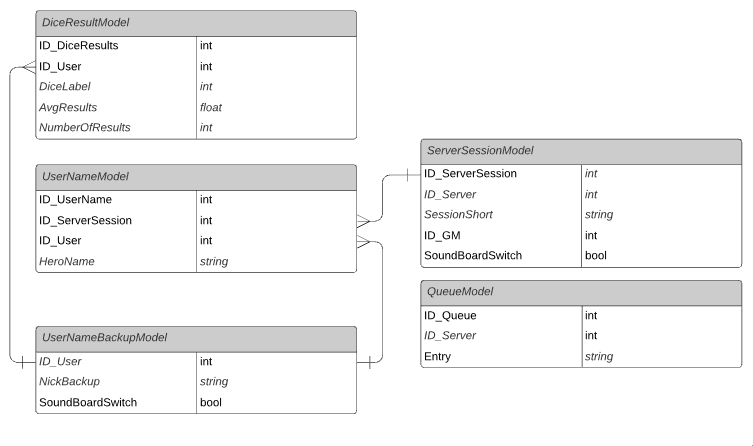
\includegraphics[width=0.90\textwidth]{dbmodels}
			\caption{Model bazy danych całej aplikacji}
		\end{figure}
	
	
		\section{Przykłady mechanizmów aplikacji}
			\subsection{Głosowanie na termin}
			Jednym z większych problemów w organizacji zarówno sesji RPG jak i innych wydarzeń w większej grupie osób jest znalezienie terminu. Jeśli organizujemy spotkanie w małej liczbie osób lub nie spotykamy się za często, ręczne sprawdzenie jest rozsądnym podejściem. Sytuacja staje się tym bardziej skomplikowana, im więcej mamy typów wydarzeń i osób do sprawdzenia. Pomysłem, który jest prosty w swoich założeniach jest utworzenie ankiety, w której uczestnicy będą głosować przy pomocy emotikon Discorda. Poźniej aplikacja użyje wyników, aby podsumować ankietę i sprawdzić kiedy można zorganizować dane wydarzenie. Przykład użycia mechanizmu został zamieszczony na Rysunku \ref{sessionPoll}.
		
			\begin{figure}[h!]
				\centering
				\begin{subfigure}[b]{.49\textwidth}
					\centering
					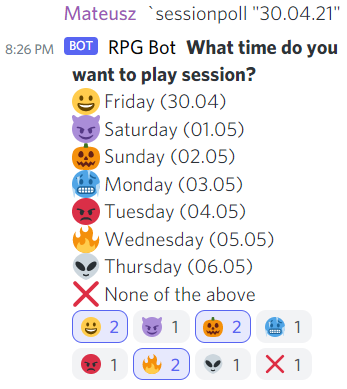
\includegraphics[width=0.93\textwidth]{poll_content}
					\caption{Ankieta oraz osiem reakcji}
				\end{subfigure}
				\hfill
				\begin{subfigure}[b]{.49\textwidth}
					\centering
					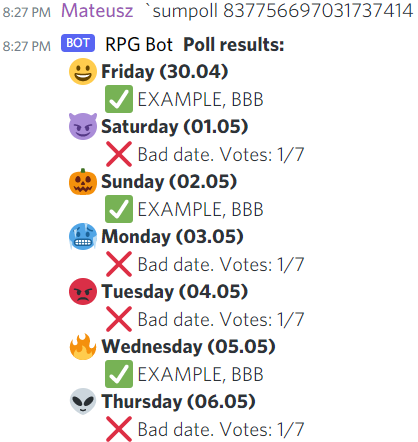
\includegraphics[width=1\textwidth]{poll_results}
					\caption{Podsumowanie ankiety}
				\end{subfigure}
				\caption{Przykład użycia mechanizmu ankiet}
				\label{sessionPoll}
			\end{figure}
	
			\subsection{Strumieniowanie muzyki z serwisu YouTube}
			Niekiedy podczas spotkania organizator chciałby odtworzyć dźwięk lub utwór muzyczny, który będzie słyszany przez wszystkich uczestników na kanale. Istnieją rozwiązania synchronizujące odtwarzacze użytkowników, jednak wymagają użycia dodatkowych mechanizmów poza Discordem\footnote{Przykładem takiego rozwiązania jest Watch2Gether (\url{https://w2g.tv}), gdzie możemy w zsynchronizowany sposób odtwarzać filmy np. z YouTube.}. Opisywana aplikacja jest w stanie odtwarzać dźwięk z serwisu YouTube na żywo na kanale głosowym (bez uprzedniego pobierania utworu), ale także umożliwia wygodne wyszukiwanie utworów poprzez czat. Przykład zastosowania mechanizmu zamieszczono na Rysunku \ref{musicBotSearch}.
	
			\begin{figure}[h!]
					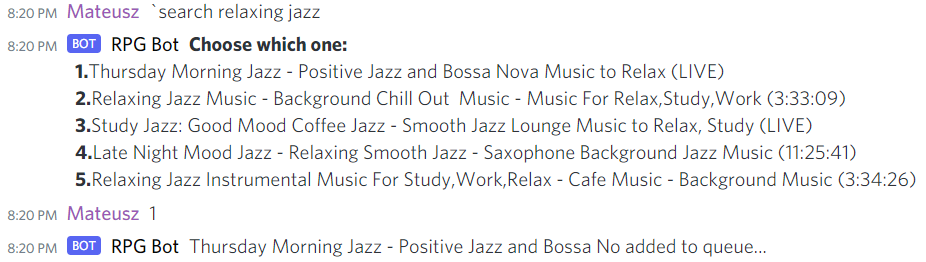
\includegraphics[width=1\textwidth]{musicExample}
					\caption{Wyszukiwanie utworów oraz wybór}
					\label{musicBotSearch}
			\end{figure}
	
			\subsection{Podsumowanie rzutów kostką po wydarzeniu}
			Aplikacja zapisuje wyniki rzutów kostką użytkowników, którzy należą do co najmniej jednej sesji. Sesja to tylko zbiór użytkowników wraz z podstawowymi informacjami o nich. System nie śledzi tego w jakiej sesji padły jakie rzuty (nie ma to sensu, ponieważ dany użytkownik nie gra więcej niż jednej sesji w danej jednostce czasu). Podsumowując rzuty korzystamy z tej struktury, aby wiedzieć jakie rzuty uwzględnić w podsumowaniu. Aby usunąć dane o rzutach, należy albo wywołać odpowiednią komendę (\texttt{`resetrolls <nameOfSession>}), lub skorzystać z komendy przywracania pseudonimów graczy po sesji (\texttt{`changenicks <nameOfSession: str> True}), która także usuwa informacje o rzutach.
			
			Zdefiniujmy sesję o nazwie \textit{Sesja\_Waterfall}, która zawiera w sobie gracza \textit{Mateusz} (\texttt{`makesession Sesja\_Waterfall 0 @Mateusz})\footnote{Konstrukcja komendy tworzenia sesji to: \texttt{`makesession <nameOfSession: str> <soundboard: bool> <*members: discord.Member>}, gdzie \texttt{nameOfSession} to nazwa sesji, \texttt{soundboard} to przełącznik reakcji dźwiękowych bota na rzuty, \texttt{members} to lista uczestników sesji.}. Po rzuceniu kilka razy kostką d100 oraz d5 (oznaczenie po literze \textit{d} to liczba ścian kostki)\footnote{W sesjach rozgrywanych na żywo 100-ścienna kostka d100 jest zastępowana przez dwie kostki. Jedna z cyfrą dziesiątek, druga z cyfrą jedności.} możemy zobaczyć średnią tych rzutów (Rysunek \ref{rollResult}).
			
			\begin{figure}[!h]
				\centering
				\begin{subfigure}[b]{.49\textwidth}
					\centering
					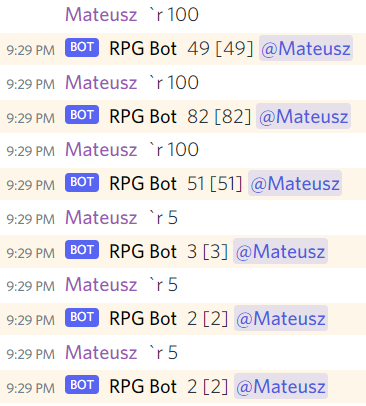
\includegraphics[width=0.93\textwidth]{rollExample}
					\caption{Kilka rzutów kostką d100 oraz d5}
				\end{subfigure}
				\hfill
				\begin{subfigure}[b]{.49\textwidth}
					\centering
					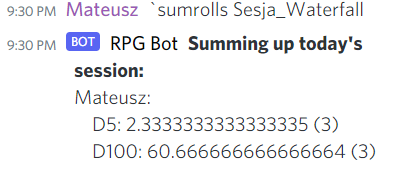
\includegraphics[width=1\textwidth]{rollsResult}
					\caption{Średni wynik po rzutach kostką}
				\end{subfigure}
				\caption{Przykładowa średnia rzutów kostką}
				\label{rollResult}
			\end{figure}
	
			Aplikacja oblicza nową średnią na podstawie wzoru i zapisuje ją z powrotem do bazy danych. Dzięki temu zużywamy minimalną ilość pamięci do spamiętywania wyników, a ilość możliwych rzutów zanim licznik się ,,przekręci'' to \(2^{63} - 1\) (maksymalna wartość pola \texttt{INTEGER} w SQLite). W praktyce bardzo trudno będzie uzyskać taką wartość podczas zwykłego użytkowania, więc jesteśmy w stanie śledzić wyniki naprawdę długich i intensywnych sesji. Przy dużej ilości rzutów coraz wyraźniej będziemy widzieć jednak zbliżanie się obliczeń do wartości oczekiwanej danej kostki i obliczanie średniej nie będzie miało sensu.
			
			\begin{center}
				\(\textrm{newAverage = } \frac{\textrm{oldAverage * oldNumberOfResults + sumOfCurrentRolls}}{\textrm{oldNumberOfResults + numberOfCurrentRolls}}\)
			\end{center}		
		
	\chapter{Inne rozwiązania}	
		Z opisanych tutaj rozwiązań korzysta wiele użytkowników na całym świecie. Są ogólnodostępne, a ich bezpłatna wersja umożliwia podstawową realizację określonych funkcji. 
		\section{YAGPDB.xyz - bot}
		Bot YAGPDB.xyz posiada funkcję rzutu kostką \(N\)-ścienną \(K\) razy dzięki komendzie \texttt{-roll}. Można również zdefiniować ile rzutów ma zostać wykonanych przez bota (-roll KdN). Udostępnia również komendę do tworzenia prostych ankiet. Nie zapisuje niestety średnich wartości rzutów wykonanych przez każdego użytkownika oraz nie udostępnia dodatkowych mechanizmów typowo pod sesję RPG. Ankiety są bardzo prostym mechanizmem, nie ma możliwości sprawdzenia pasującego terminu dla określonej sesji. \url{https://yagpdb.xyz/}
		\section{Rhytm - bot}
		Rhytm to najbardziej popularny bot muzyczny, obsługujący zarówno muzykę z URL YouTube, jak i wyszukiwanie utworów poprzez czat Discorda. Prowadzi kolejkę odtwarzania oraz wszelkie mechanizmy niezbędne dla odtwarzacza muzycznego. Służy tylko odtwarzaniu muzyki, nie posiada innych mechanizmów związanych z sesjami RPG. Opcjonalnie może służyć jako drugi bot do odtwarzania dźwięków (boty mogą odtwarzać na raz tylko jedno źródło dźwięku). \url{https://rythm.fm/}
		\section{Roll20 - serwis internetowy}
		Serwis Roll20 jest stworzony z myślą o prowadzeniu oraz rozgrywaniu sesji RPG. W podstawowej, bezpłatnej wersji umożliwia rzuty kostką, prowadzenie kart postaci oraz dużo więcej. Jest jednak dodatkowym serwisem (jeśli użytkownik używa Discorda do porozumiewania się), który każdy z graczy musi regularnie sprawdzać i odpowiednio ustawiać. Nie ma również możliwości zagłosowania na termin organizowanej sesji. Wiele graczy zgłaszało, że lepiej im prowadzić kartę postaci w pliku pdf na komputerze lub na kartce papieru, niż na powyższym serwisie. \url{https://app.roll20.net}
		\section{Watch2Gether - serwis internetowy}
		Mówiąc o wspólnym słuchaniu muzyki czy podkładu dźwiękowego nie można pominąć jednego z najpopularniejszych rozwiązań przystosowanych do tego celu, czyli Watch2Gether. Rozwiązanie umożliwia odtwarzanie filmów z wielu popularnych takich jak YouTube czy Vimeo. Oferuje utworzenie pokoju dla słuchających oraz listy odtwarzania, do której każdy z uczestników może dodawać swoje propozycje. Może zostać użyty do wspólnego słuchania ścieżki dźwiękowej, synchronizując odtwarzacze użytkowników. Niestety na tym kończy się funkcjonalność przydatna w realizacji rozgrywek. Nie uświadczymy żadnego wsparcia dla rzutów kostką czy też zarządzaniem użytkownikami. Poza tym, w wersji mobilnej strona musi być cały czas aktywna, aby odtwarzać dźwięk. Przełączenie się na inną aplikację automatycznie wyłącza odtwarzany film. To uniemożliwia rozgrywkę w jakikolwiek sposób angażując tylko jedno urządzenie. 
		\section{Foundry Virtual Tabletop - serwis internetowy}
		Foundry Virtual Tabletop jest rozwiązaniem z wyglądu bardzo przypominającym serwis Roll20. Wymaga jednak uiszczenia jednorazowej opłaty na dostęp do serwera przez Mistrza Gry (gracze łączą się za darmo) w wysokości około 61.50 USD. Rozwiązanie bardzo zaawansowane, posiadające gotowe grafiki, mapy czy karty postaci nawiązujące do najpopularniejszych systemów RPG. Niestety potrzeba dłuższego czasu na zapoznanie się z interfejsem oraz możliwościami, co dla nowych i mało doświadczonych graczy będzie stanowiło sporą przeszkodę. Wersja demonstracyjna zamieszczona na stronie produktu nie pozwala na dużo, przez co trudno w pełni ocenić praktyczność i jakość tego projektu. \url{https://foundryvtt.com/}
		
	\chapter{Podsumowanie}
	Istotą niniejszej pracy inżynierskiej była implementacja mechanizmów znacznie upraszczających rozgrywanie sesji gier fabularnych, ale też organizację spotkań w dużej grupie osób. Było to możliwe dzięki zastosowaniu popularnego i przystępnego komunikatora Discord, biblioteki discord dla języka Python korzystającej z podejścia asynchronicznego, jak również SQLAlchemy, będącego systemem ORM bazy danych SQLite. W toku trwania prac nad projektem wytworzono sprawnie działający system, którego użycie nie powinno sprawiać problemów po krótkim zapoznaniu. Każda funkcjonalność jest odpowiednio opisana w kodzie źródłowym, ale również w komendzie \texttt{`help}, dostępnej publicznie dla użytkownika.  przypadku wystąpienia nieoczekiwanego przez autora programu błędu, bot nie przestaje działać, ale wypisuje stosowną informację na czacie, oraz w logach. Aplikacja może zostać użyta również przez organizatorów wydarzeń niezwiązanych tematycznie z grami RPG. Mechanizm zarządzania użytkownikami na kanale czy tworzenie ankiet służących wyborowi konkretnego terminu spotkania to przykłady funkcjonalności o dużo szerszym zastosowaniu. Zapotrzebowanie na taką aplikację powstało głównie w wyniku głosów użytkowników rozgrywających gry fabularne, ale także braku dostatecznie funkcjonalnych rozwiązań na rynku.
	
		\section{Analiza realizacji celów pracy}
		Wytworzone rozwiązanie spełnia założone na początku pracy cele oraz pokrywa przewidziany zakres pracy (wstęp dokumentu):
		\begin{enumerate}
			\item Komenda \texttt{`roll} losuje liczbę z wybranego przez użytkownika przedziału w sposób losowy, wykorzystując funkcję z biblioteki \texttt{random} języka Python/
			\item Moduł \texttt{Rolls} zbiera informacje o rzutach graczy oraz umożliwia podsumowanie wyników.
			\item Moduł \texttt{Soundboard} służy odtwarzaniu dźwięków oraz muzyki (również na żywo z serwisu YouTube, bez uprzedniego pobierania całości).
			\item Komenda \texttt{`changenicks} zmienia pseudonimy graczy na odpowiednie dla danej sesji.
			\item Moduł \texttt{Session} realizuje funkcjonalności drużyn graczy. Wyciszanie oraz przenoszenie użytkowników na inne kanały jest również możliwe.
			\item Rzuty kostką realizowane przez moduł \texttt{Rolls} posiada możliwość przypisania użytkownika (dodatkowy argument), który otrzyma informację o rzucie.
			\item Dźwiękowa reakcja bota na korzystny lub niekorzystny wynik na kostce został zaimplementowany w module \texttt{Rolls}. Możliwość wyłączenia tej funkcjonalności została odzwierciedlona w odpowiednim argumencie komendy tworzenia sesji.
			\item Kolejka odtwarzania dla danego serwera jest przechowywana w bazie danych i aktualizowana na bieżąco przy zmianie utworu oraz modyfikacji kolejki.
			\item Komenda \texttt{`sessionpoll} umożliwia tworzenie ankiet dla użytkowników, wraz z komendą \texttt{`sumpoll}, podsumowującą wyniki ankiety.
		\end{enumerate}
	
		\section{Dalsze plany na rozwój aplikacji} 
	 	Kolejnym celem na rozwój jest przede wszystkim zastosowanie obiektów typu \texttt{Embed} zamiast zwykłych wiadomości na czacie. Takie prezentowanie treści jest dużo lepsze oraz czytelniejsze w odbiorze dla użytkownika. Ilość pól oraz ich rozmieszczenie w wiadomości jest dowolne. Przykład takiego obiektu wysłanego na czacie zamieszczono na Rysunku \ref{embedexample}.
	 	\begin{figure}[h]
	 		\centering
	 		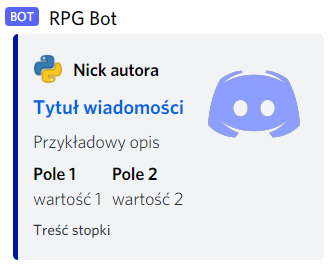
\includegraphics{embed}
	 		\caption{Przykład wiadomości typu \texttt{Embed}}
	 		\label{embedexample}
	 	\end{figure}
	 	
	 	W celu wydajnego działania na większej ilości serwerów oraz oszczędzania zasobów należy także zoptymalizować działanie modułu muzycznego. Odtwarzanie dźwięków na pustym kanale oraz połączenie z takim kanałem powinny zostać wykluczone, co może mieć duże znaczenie podczas znacznego obciążenia aplikacji. Aby sprawniej zarządzać sesjami oraz użytkownikami, przydatny mógłby być interfejs zaimplementowany w formie graficznej, np. w przeglądarce. Zamiast wpisywania komend, użytkownik mógłby część funkcji wywołać przy pomocy elementów graficznych. To umożliwiłoby również przechowywanie całych kart postaci oraz wygodne zarządzanie nimi (przy obecnym interfejsie prowadzenie karty postaci jest zbyt żmudne). Jednym z ostatnich kroków rozwoju dla aplikacji jest udostępnienie jej dla szerszej publiczności na publicznym hostingu, aby każdy użytkownik Discorda mógł dodać bota na swój własny serwer i korzystać z niego niezależnie od uruchomionego lokalnie skryptu.
	 	
	 	\section{Wnioski}
	 	Dzięki przygotowaniu projektu RPGamer poznałem proces tworzenia aplikacji z zupełnie innej perspektywy. Przede wszystkim dzięki braku z góry narzuconych celów czy specyfikacji, musiałem głęboko zastanowić się czy proponowane przeze mnie rozwiązania będą praktyczne i użyteczne dla przeciętnego użytkownika. Należało przeprowadzić analizę najbardziej potrzebnych mechanizmów oraz zaimplementować je, używając gotowych rozwiązań proponowanych przez aplikację Discorda. 
	 	
	 	Dużą nowością dla mnie było podejście asynchroniczne w tworzeniu kodu. Musiałem zwracać uwagę na to czy dana metoda nie wykonuje się zbyt długo i nie blokuje wykonania innych metod. Także przy korzystaniu z zewnętrznych bibliotek, trzeba było uważać na ich blokujące wywołania (np. przy pobieraniu danych z serwisu YouTube przez youtube\_dl).
	 	
	 	Z uwagi na wielkość projektu i dużą liczbę metod oraz aspektów, którym należało poświęcić czas nauczyłem się również priorytetyzować zadania do wykonania. Zaadaptowałem nie stosowany przeze mnie wcześniej sposób pracy, jakim jest podział zadań według poziomu istotności z punktu widzenia działania projektu. Stworzyłem tablicę na stronie Monday\footnote{\url{https://www.monday.com}}, na której każde zadanie było klasyfikowane do jednej z trzech kategorii: \textit{Crucial}, \textit{Medium crucial} oraz \textit{Feature}. Przed każdą sesją tworzenia kodu podsumowywałem to jakie cele zostały do zrealizowania oraz czym zająć się w następnej kolejności. Pozwoliło to na sprawną i dokładną pracę nad najbardziej istotnymi częściami bota, a części mogące stanowić jedynie dodatek nie wpływający znacznie na funkcjonalność pozostawić do poprawy w ewentualnych kolejnych wersjach aplikacji.
	 
	\setcounter{tocdepth}{1}
	\listoffigures
	\addcontentsline{toc}{chapter}{Spis rysunków}
	\lstlistoflistings	
	\addcontentsline{toc}{chapter}{Listingi}
	\printbibliography[title=Bibliografia]
	\addcontentsline{toc}{chapter}{Bibliografia}
\end{document}
